\documentclass{standalone}
\usepackage{tikz}
\usetikzlibrary{patterns, positioning}

\begin{document}
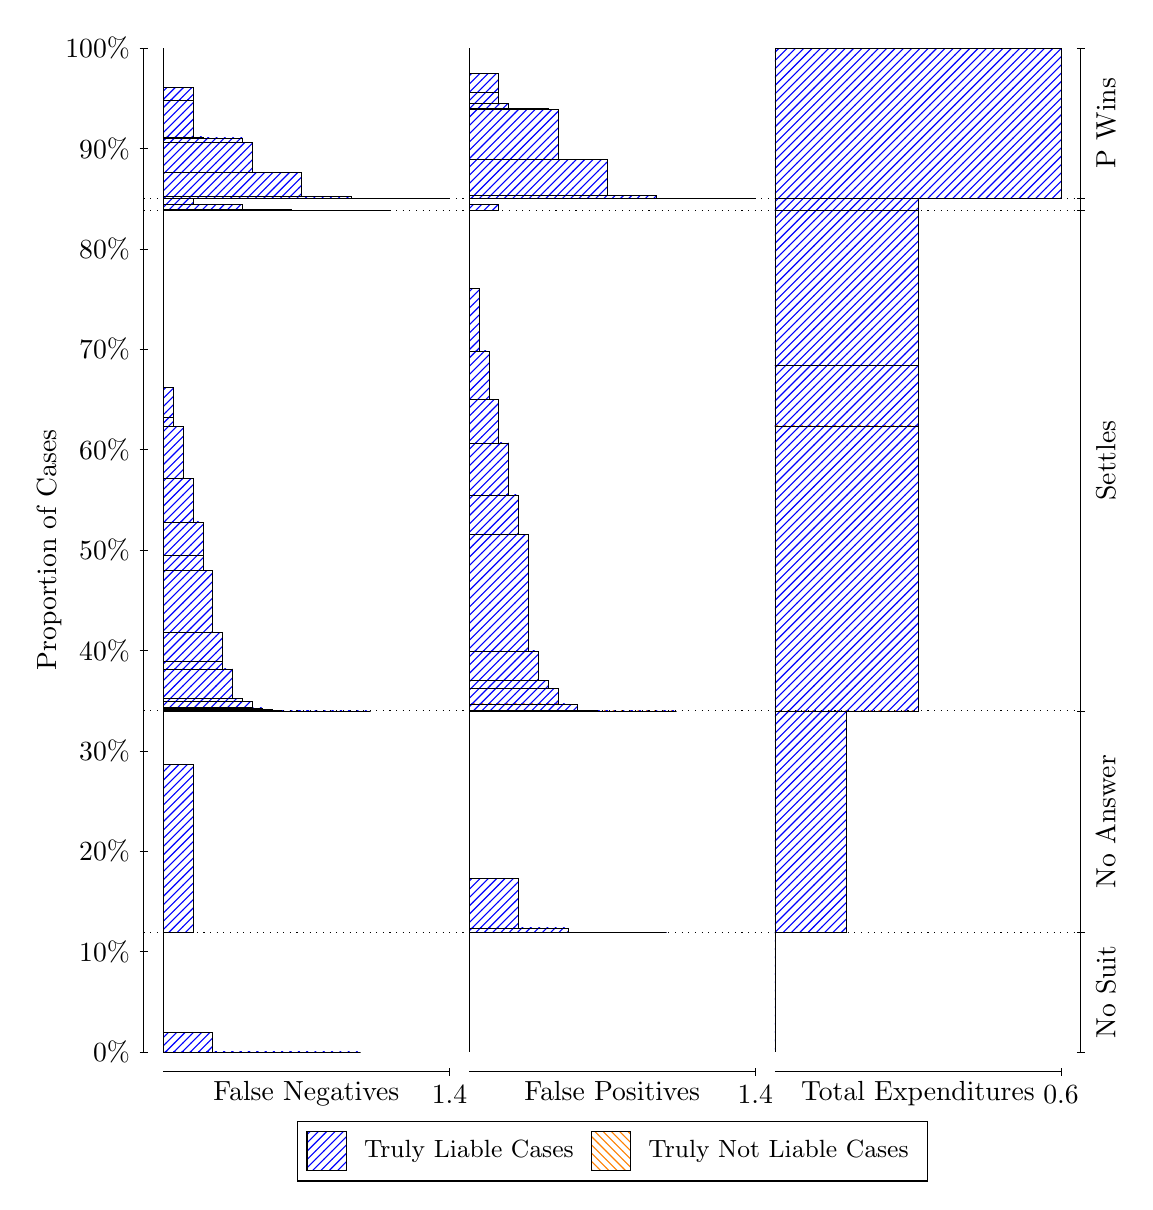
\begin{tikzpicture}
\draw[black, very thin] (1.5,1.75) -- (1.5,14.5);
\node[rotate=90, anchor=center] at (0.3, 8.125) {Proportion of Cases};
\draw[black, very thin] (1.45,1.75) -- (1.55,1.75);
\node[anchor=east] at (1.45, 1.75) {0\%};
\draw[black, very thin] (1.45,3.025) -- (1.55,3.025);
\node[anchor=east] at (1.45, 3.025) {10\%};
\draw[black, very thin] (1.45,4.3) -- (1.55,4.3);
\node[anchor=east] at (1.45, 4.3) {20\%};
\draw[black, very thin] (1.45,5.575) -- (1.55,5.575);
\node[anchor=east] at (1.45, 5.575) {30\%};
\draw[black, very thin] (1.45,6.85) -- (1.55,6.85);
\node[anchor=east] at (1.45, 6.85) {40\%};
\draw[black, very thin] (1.45,8.125) -- (1.55,8.125);
\node[anchor=east] at (1.45, 8.125) {50\%};
\draw[black, very thin] (1.45,9.4) -- (1.55,9.4);
\node[anchor=east] at (1.45, 9.4) {60\%};
\draw[black, very thin] (1.45,10.675) -- (1.55,10.675);
\node[anchor=east] at (1.45, 10.675) {70\%};
\draw[black, very thin] (1.45,11.95) -- (1.55,11.95);
\node[anchor=east] at (1.45, 11.95) {80\%};
\draw[black, very thin] (1.45,13.225) -- (1.55,13.225);
\node[anchor=east] at (1.45, 13.225) {90\%};
\draw[black, very thin] (1.45,14.5) -- (1.55,14.5);
\node[anchor=east] at (1.45, 14.5) {100\%};

\draw[black, very thin] (13.4,1.75) -- (13.4,14.5);
\draw[black, very thin] (13.35,1.75) -- (13.45,1.75);
\node[anchor=west] at (13.35, 1.75) {};
\draw[black, very thin] (13.35,3.2697) -- (13.45,3.2697);
\node[anchor=west] at (13.35, 3.2697) {};
\draw[black, very thin] (13.35,6.0815) -- (13.45,6.0815);
\node[anchor=west] at (13.35, 6.0815) {};
\draw[black, very thin] (13.35,12.44) -- (13.45,12.44);
\node[anchor=west] at (13.35, 12.44) {};
\draw[black, very thin] (13.35,12.592) -- (13.45,12.592);
\node[anchor=west] at (13.35, 12.592) {};
\draw[black, very thin] (13.35,14.5) -- (13.45,14.5);
\node[anchor=west] at (13.35, 14.5) {};

\draw[black, very thin, pattern color=blue, pattern=north east lines] (1.75,1.75) rectangle (4.2557,1.75);
\draw[black, very thin, pattern color=blue, pattern=north east lines] (1.75,1.75) rectangle (3.6293,1.75);
\draw[black, very thin, pattern color=blue, pattern=north east lines] (1.75,1.75) rectangle (3.0029,1.7521);
\draw[black, very thin, pattern color=blue, pattern=north east lines] (1.75,1.7521) rectangle (2.3764,1.9988);
\draw[black, very thin, pattern color=orange, pattern=north west lines] (1.75,1.9988) rectangle (1.75,1.9988);
\draw[black, very thin, pattern color=blue, pattern=north east lines] (1.75,1.9988) rectangle (1.75,3.2697);
\draw[black, very thin, pattern color=blue, pattern=north east lines] (1.75,3.2697) rectangle (2.1259,5.4001);
\draw[black, very thin, pattern color=orange, pattern=north west lines] (1.75,5.4001) rectangle (1.75,5.4001);
\draw[black, very thin, pattern color=blue, pattern=north east lines] (1.75,5.4001) rectangle (1.75,6.0815);
\draw[black, very thin, pattern color=blue, pattern=north east lines] (1.75,6.0815) rectangle (4.381,6.0815);
\draw[black, very thin, pattern color=blue, pattern=north east lines] (1.75,6.0815) rectangle (4.1305,6.0815);
\draw[black, very thin, pattern color=blue, pattern=north east lines] (1.75,6.0815) rectangle (3.8799,6.0815);
\draw[black, very thin, pattern color=blue, pattern=north east lines] (1.75,6.0815) rectangle (3.7546,6.0815);
\draw[black, very thin, pattern color=blue, pattern=north east lines] (1.75,6.0815) rectangle (3.6293,6.0815);
\draw[black, very thin, pattern color=blue, pattern=north east lines] (1.75,6.0815) rectangle (3.504,6.0817);
\draw[black, very thin, pattern color=blue, pattern=north east lines] (1.75,6.0817) rectangle (3.3787,6.0817);
\draw[black, very thin, pattern color=blue, pattern=north east lines] (1.75,6.0817) rectangle (3.2534,6.0915);
\draw[black, very thin, pattern color=blue, pattern=north east lines] (1.75,6.0915) rectangle (3.1282,6.1043);
\draw[black, very thin, pattern color=blue, pattern=north east lines] (1.75,6.1043) rectangle (3.0029,6.1195);
\draw[black, very thin, pattern color=blue, pattern=north east lines] (1.75,6.1195) rectangle (2.8776,6.1234);
\draw[black, very thin, pattern color=blue, pattern=north east lines] (1.75,6.1234) rectangle (2.8776,6.205);
\draw[black, very thin, pattern color=blue, pattern=north east lines] (1.75,6.205) rectangle (2.7523,6.238);
\draw[black, very thin, pattern color=blue, pattern=north east lines] (1.75,6.238) rectangle (2.627,6.6149);
\draw[black, very thin, pattern color=blue, pattern=north east lines] (1.75,6.6149) rectangle (2.5017,6.7078);
\draw[black, very thin, pattern color=blue, pattern=north east lines] (1.75,6.7078) rectangle (2.5017,7.0772);
\draw[black, very thin, pattern color=blue, pattern=north east lines] (1.75,7.0772) rectangle (2.3764,7.8666);
\draw[black, very thin, pattern color=blue, pattern=north east lines] (1.75,7.8666) rectangle (2.2511,8.0612);
\draw[black, very thin, pattern color=blue, pattern=north east lines] (1.75,8.0612) rectangle (2.2511,8.4816);
\draw[black, very thin, pattern color=blue, pattern=north east lines] (1.75,8.4816) rectangle (2.1259,9.0366);
\draw[black, very thin, pattern color=blue, pattern=north east lines] (1.75,9.0366) rectangle (2.0006,9.6957);
\draw[black, very thin, pattern color=blue, pattern=north east lines] (1.75,9.6957) rectangle (2.0006,9.6957);
\draw[black, very thin, pattern color=blue, pattern=north east lines] (1.75,9.6957) rectangle (1.8753,9.8056);
\draw[black, very thin, pattern color=blue, pattern=north east lines] (1.75,9.8056) rectangle (1.8753,10.195);
\draw[black, very thin, pattern color=orange, pattern=north west lines] (1.75,10.195) rectangle (1.75,10.195);
\draw[black, very thin, pattern color=blue, pattern=north east lines] (1.75,10.195) rectangle (1.75,12.44);
\draw[black, very thin, pattern color=blue, pattern=north east lines] (1.75,12.44) rectangle (4.6316,12.44);
\draw[black, very thin, pattern color=blue, pattern=north east lines] (1.75,12.44) rectangle (4.0052,12.44);
\draw[black, very thin, pattern color=blue, pattern=north east lines] (1.75,12.44) rectangle (3.3787,12.448);
\draw[black, very thin, pattern color=blue, pattern=north east lines] (1.75,12.448) rectangle (2.7523,12.515);
\draw[black, very thin, pattern color=blue, pattern=north east lines] (1.75,12.515) rectangle (2.1259,12.592);
\draw[black, very thin, pattern color=orange, pattern=north west lines] (1.75,12.592) rectangle (1.75,12.592);
\draw[black, very thin, pattern color=blue, pattern=north east lines] (1.75,12.592) rectangle (5.3833,12.592);
\draw[black, very thin, pattern color=blue, pattern=north east lines] (1.75,12.592) rectangle (4.7569,12.592);
\draw[black, very thin, pattern color=blue, pattern=north east lines] (1.75,12.592) rectangle (4.1305,12.617);
\draw[black, very thin, pattern color=blue, pattern=north east lines] (1.75,12.617) rectangle (4.0052,12.617);
\draw[black, very thin, pattern color=blue, pattern=north east lines] (1.75,12.617) rectangle (3.504,12.916);
\draw[black, very thin, pattern color=blue, pattern=north east lines] (1.75,12.916) rectangle (3.3787,12.916);
\draw[black, very thin, pattern color=blue, pattern=north east lines] (1.75,12.916) rectangle (2.8776,13.297);
\draw[black, very thin, pattern color=blue, pattern=north east lines] (1.75,13.297) rectangle (2.7523,13.359);
\draw[black, very thin, pattern color=blue, pattern=north east lines] (1.75,13.359) rectangle (2.2511,13.372);
\draw[black, very thin, pattern color=blue, pattern=north east lines] (1.75,13.372) rectangle (2.1259,13.84);
\draw[black, very thin, pattern color=blue, pattern=north east lines] (1.75,13.84) rectangle (2.1259,14.005);
\draw[black, very thin, pattern color=orange, pattern=north west lines] (1.75,14.005) rectangle (1.75,14.005);
\draw[black, very thin, pattern color=blue, pattern=north east lines] (1.75,14.005) rectangle (1.75,14.5);
\draw[black, very thin, pattern color=orange, pattern=north west lines] (5.6333,1.75) rectangle (5.6333,1.75);
\draw[black, very thin, pattern color=blue, pattern=north east lines] (5.6333,1.75) rectangle (5.6333,3.2697);
\draw[black, very thin, pattern color=orange, pattern=north west lines] (5.6333,3.2697) rectangle (8.1391,3.2697);
\draw[black, very thin, pattern color=blue, pattern=north east lines] (5.6333,3.2697) rectangle (8.1391,3.2697);
\draw[black, very thin, pattern color=blue, pattern=north east lines] (5.6333,3.2697) rectangle (7.5126,3.2701);
\draw[black, very thin, pattern color=blue, pattern=north east lines] (5.6333,3.2701) rectangle (6.8862,3.3251);
\draw[black, very thin, pattern color=blue, pattern=north east lines] (5.6333,3.3251) rectangle (6.2598,3.9511);
\draw[black, very thin, pattern color=blue, pattern=north east lines] (5.6333,3.9511) rectangle (5.6333,6.0815);
\draw[black, very thin, pattern color=orange, pattern=north west lines] (5.6333,6.0815) rectangle (8.2644,6.0815);
\draw[black, very thin, pattern color=blue, pattern=north east lines] (5.6333,6.0815) rectangle (8.2644,6.0815);
\draw[black, very thin, pattern color=orange, pattern=north west lines] (5.6333,6.0815) rectangle (8.0138,6.0815);
\draw[black, very thin, pattern color=blue, pattern=north east lines] (5.6333,6.0815) rectangle (8.0138,6.0815);
\draw[black, very thin, pattern color=orange, pattern=north west lines] (5.6333,6.0815) rectangle (7.7632,6.0815);
\draw[black, very thin, pattern color=blue, pattern=north east lines] (5.6333,6.0815) rectangle (7.7632,6.0815);
\draw[black, very thin, pattern color=blue, pattern=north east lines] (5.6333,6.0815) rectangle (7.6379,6.0816);
\draw[black, very thin, pattern color=orange, pattern=north west lines] (5.6333,6.0816) rectangle (7.5126,6.0816);
\draw[black, very thin, pattern color=blue, pattern=north east lines] (5.6333,6.0816) rectangle (7.5126,6.0816);
\draw[black, very thin, pattern color=blue, pattern=north east lines] (5.6333,6.0816) rectangle (7.3874,6.0816);
\draw[black, very thin, pattern color=orange, pattern=north west lines] (5.6333,6.0816) rectangle (7.2621,6.0816);
\draw[black, very thin, pattern color=blue, pattern=north east lines] (5.6333,6.0816) rectangle (7.2621,6.086);
\draw[black, very thin, pattern color=blue, pattern=north east lines] (5.6333,6.086) rectangle (7.1368,6.0863);
\draw[black, very thin, pattern color=orange, pattern=north west lines] (5.6333,6.0863) rectangle (7.0115,6.0863);
\draw[black, very thin, pattern color=blue, pattern=north east lines] (5.6333,6.0863) rectangle (7.0115,6.1684);
\draw[black, very thin, pattern color=blue, pattern=north east lines] (5.6333,6.1684) rectangle (6.8862,6.1693);
\draw[black, very thin, pattern color=blue, pattern=north east lines] (5.6333,6.1693) rectangle (6.7609,6.1695);
\draw[black, very thin, pattern color=orange, pattern=north west lines] (5.6333,6.1695) rectangle (6.7609,6.1695);
\draw[black, very thin, pattern color=blue, pattern=north east lines] (5.6333,6.1695) rectangle (6.7609,6.366);
\draw[black, very thin, pattern color=blue, pattern=north east lines] (5.6333,6.366) rectangle (6.6356,6.4715);
\draw[black, very thin, pattern color=orange, pattern=north west lines] (5.6333,6.4715) rectangle (6.5103,6.4715);
\draw[black, very thin, pattern color=blue, pattern=north east lines] (5.6333,6.4715) rectangle (6.5103,6.8444);
\draw[black, very thin, pattern color=blue, pattern=north east lines] (5.6333,6.8444) rectangle (6.3851,8.3265);
\draw[black, very thin, pattern color=orange, pattern=north west lines] (5.6333,8.3265) rectangle (6.2598,8.3265);
\draw[black, very thin, pattern color=blue, pattern=north east lines] (5.6333,8.3265) rectangle (6.2598,8.8254);
\draw[black, very thin, pattern color=blue, pattern=north east lines] (5.6333,8.8254) rectangle (6.1345,8.8254);
\draw[black, very thin, pattern color=blue, pattern=north east lines] (5.6333,8.8254) rectangle (6.1345,9.4845);
\draw[black, very thin, pattern color=blue, pattern=north east lines] (5.6333,9.4845) rectangle (6.0092,10.04);
\draw[black, very thin, pattern color=blue, pattern=north east lines] (5.6333,10.04) rectangle (5.8839,10.655);
\draw[black, very thin, pattern color=blue, pattern=north east lines] (5.6333,10.655) rectangle (5.7586,11.444);
\draw[black, very thin, pattern color=blue, pattern=north east lines] (5.6333,11.444) rectangle (5.6333,12.44);
\draw[black, very thin, pattern color=orange, pattern=north west lines] (5.6333,12.44) rectangle (6.0092,12.44);
\draw[black, very thin, pattern color=blue, pattern=north east lines] (5.6333,12.44) rectangle (6.0092,12.517);
\draw[black, very thin, pattern color=blue, pattern=north east lines] (5.6333,12.517) rectangle (5.6333,12.592);
\draw[black, very thin, pattern color=orange, pattern=north west lines] (5.6333,12.592) rectangle (9.2667,12.592);
\draw[black, very thin, pattern color=blue, pattern=north east lines] (5.6333,12.592) rectangle (9.2667,12.592);
\draw[black, very thin, pattern color=orange, pattern=north west lines] (5.6333,12.592) rectangle (8.6402,12.592);
\draw[black, very thin, pattern color=blue, pattern=north east lines] (5.6333,12.592) rectangle (8.6402,12.592);
\draw[black, very thin, pattern color=orange, pattern=north west lines] (5.6333,12.592) rectangle (8.0138,12.592);
\draw[black, very thin, pattern color=blue, pattern=north east lines] (5.6333,12.592) rectangle (8.0138,12.63);
\draw[black, very thin, pattern color=orange, pattern=north west lines] (5.6333,12.63) rectangle (7.3874,12.63);
\draw[black, very thin, pattern color=blue, pattern=north east lines] (5.6333,12.63) rectangle (7.3874,13.086);
\draw[black, very thin, pattern color=orange, pattern=north west lines] (5.6333,13.086) rectangle (7.2621,13.086);
\draw[black, very thin, pattern color=blue, pattern=north east lines] (5.6333,13.086) rectangle (7.2621,13.087);
\draw[black, very thin, pattern color=blue, pattern=north east lines] (5.6333,13.087) rectangle (6.7609,13.72);
\draw[black, very thin, pattern color=orange, pattern=north west lines] (5.6333,13.72) rectangle (6.6356,13.72);
\draw[black, very thin, pattern color=blue, pattern=north east lines] (5.6333,13.72) rectangle (6.6356,13.734);
\draw[black, very thin, pattern color=blue, pattern=north east lines] (5.6333,13.734) rectangle (6.1345,13.795);
\draw[black, very thin, pattern color=blue, pattern=north east lines] (5.6333,13.795) rectangle (6.0092,13.937);
\draw[black, very thin, pattern color=orange, pattern=north west lines] (5.6333,13.937) rectangle (6.0092,13.937);
\draw[black, very thin, pattern color=blue, pattern=north east lines] (5.6333,13.937) rectangle (6.0092,14.176);
\draw[black, very thin, pattern color=blue, pattern=north east lines] (5.6333,14.176) rectangle (5.6333,14.5);
\draw[black, very thin, pattern color=orange, pattern=north west lines] (9.5167,1.75) rectangle (9.5167,1.75);
\draw[black, very thin, pattern color=blue, pattern=north east lines] (9.5167,1.75) rectangle (9.5167,3.2697);
\draw[black, very thin, pattern color=orange, pattern=north west lines] (9.5167,3.2697) rectangle (10.425,3.2697);
\draw[black, very thin, pattern color=blue, pattern=north east lines] (9.5167,3.2697) rectangle (10.425,6.0815);
\draw[black, very thin, pattern color=orange, pattern=north west lines] (9.5167,6.0815) rectangle (11.333,6.0815);
\draw[black, very thin, pattern color=blue, pattern=north east lines] (9.5167,6.0815) rectangle (11.333,9.7025);
\draw[black, very thin, pattern color=orange, pattern=north west lines] (9.5167,9.7025) rectangle (11.333,9.7025);
\draw[black, very thin, pattern color=blue, pattern=north east lines] (9.5167,9.7025) rectangle (11.333,10.473);
\draw[black, very thin, pattern color=orange, pattern=north west lines] (9.5167,10.473) rectangle (11.333,10.473);
\draw[black, very thin, pattern color=blue, pattern=north east lines] (9.5167,10.473) rectangle (11.333,12.44);
\draw[black, very thin, pattern color=orange, pattern=north west lines] (9.5167,12.44) rectangle (11.333,12.44);
\draw[black, very thin, pattern color=blue, pattern=north east lines] (9.5167,12.44) rectangle (11.333,12.592);
\draw[black, very thin, pattern color=orange, pattern=north west lines] (9.5167,12.592) rectangle (13.15,12.592);
\draw[black, very thin, pattern color=blue, pattern=north east lines] (9.5167,12.592) rectangle (13.15,14.5);
\draw[black, dotted] (1.5,3.2697) -- (13.4,3.2697);
\draw[black, dotted] (1.5,6.0815) -- (13.4,6.0815);
\draw[black, dotted] (1.5,12.44) -- (13.4,12.44);
\draw[black, dotted] (1.5,12.592) -- (13.4,12.592);
\draw[black, very thin] (1.75,1.5) -- (5.3833,1.5);
\node[anchor=north] at (3.5667, 1.5) {False Negatives};
\draw[black, very thin] (5.3833,1.45) -- (5.3833,1.55);
\node[anchor=north] at (5.3833, 1.45) {1.4};

\draw[black, very thin] (5.6333,1.5) -- (9.2667,1.5);
\node[anchor=north] at (7.45, 1.5) {False Positives};
\draw[black, very thin] (9.2667,1.45) -- (9.2667,1.55);
\node[anchor=north] at (9.2667, 1.45) {1.4};

\draw[black, very thin] (9.5167,1.5) -- (13.15,1.5);
\node[anchor=north] at (11.333, 1.5) {Total Expenditures};
\draw[black, very thin] (13.15,1.45) -- (13.15,1.55);
\node[anchor=north] at (13.15, 1.45) {0.6};

\node[black, centered, rotate=90] at (13.72, 2.5098) {No Suit};
\node[black, centered, rotate=90] at (13.72, 4.6756) {No Answer};
\node[black, centered, rotate=90] at (13.72, 9.2606) {Settles};

\node[black, centered, rotate=90] at (13.72, 13.546) {P Wins};

\draw (7.449999999999999,1.5) node[draw=none] (baseCoordinate) {};
\begin{scope}[align=center]
        \matrix[scale=0.5, draw=black, below=0.5cm of baseCoordinate, nodes={draw}, column sep=0.1cm]{
            \node[rectangle, draw, minimum width=0.5cm, minimum height=0.5cm, pattern=north east lines, pattern color=blue] {}; &
            \node[draw=none, font=\small] (B) {Truly Liable Cases}; &
            \node[rectangle, draw, minimum width=0.5cm, minimum height=0.5cm, pattern=north west lines, pattern color=orange] {}; &
            \node[draw=none, font=\small] (B) {Truly Not Liable Cases}; \\
            };
\end{scope}

\end{tikzpicture}
\end{document}